\documentclass[main.tex]{subfiles}
\begin{document}

\chapter{Oefenzittingen}
\label{cha:oefenzittingen}

\section{Oefenzitting 1}
\label{sec:oefenzitting-1}

\subsection*{Vraag 1}
Inderdaad, zie \ref{omgekeerde-reguliere-taal-is-regulier}.

\subsection*{Vraag 2}
\begin{enumerate}
\item
  \[ (\epsilon|1(01)^{*}) \]

  \begin{figure}[H]
    \centering
    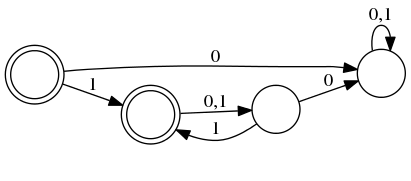
\includegraphics[width=0.5\textwidth]{assets/oz1v2-1.png}
    \caption{NFA vraag 2 deel 1}
    \label{fig:oz1v2-1}
  \end{figure}

\item
  \[ ((0^{*}00(\epsilon|1)0^{*})|(0^{*}0(\epsilon|1)00^{*})|(0^{*}(\epsilon|1)000^{*})) \]
  \begin{figure}[H]
    \centering
    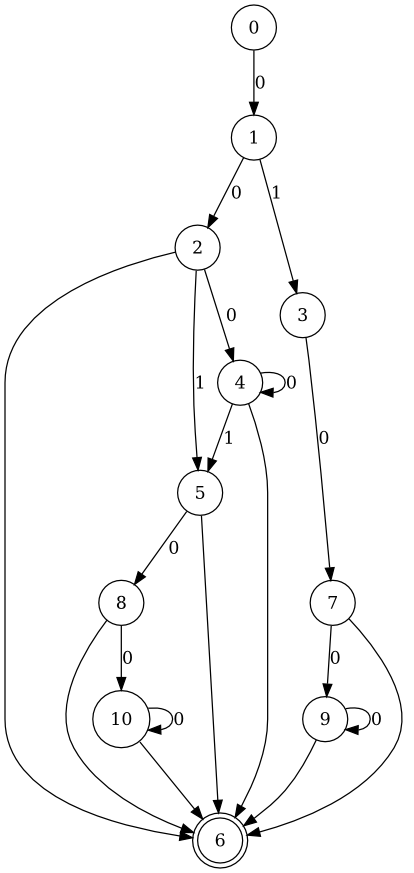
\includegraphics[width=0.3\textwidth]{assets/oz1v2-2.png}
    \caption{NFA vraag 2 deel 2}
    \label{fig:oz1v2-2}
  \end{figure}

\item 
  \[ (\epsilon|0|1|00|01|10||001|010|011|100|101|110(0|1)^{*}|1110(1|0)^{*}|1111(1|0)^{*}) \]
  \begin{figure}[H]
    \centering
    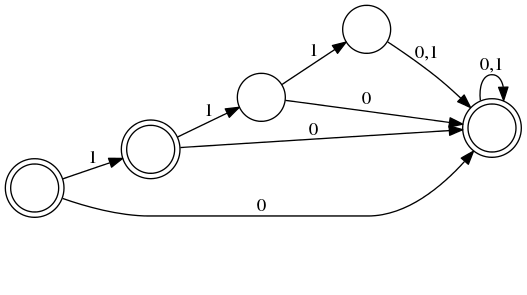
\includegraphics[width=0.5\textwidth]{assets/oz1v2-3.png}
    \caption{NFA vraag 2 deel 3}
    \label{fig:oz1v2-3}
  \end{figure}

\item Onmogelijk, dat is geen reguliere taal.
\end{enumerate}

\subsection*{Vraag 3}
Geen idee.
\question{vragen in oefenzitting}



\end{document}
